\documentclass{article}

% Pacotes
\usepackage[utf8]{inputenc}
\usepackage[T1]{fontenc}
\usepackage[brazil]{babel}
\usepackage{graphicx}
\usepackage{amsmath, amssymb}
\usepackage{geometry}
\usepackage{setspace}
\usepackage{indentfirst}
\usepackage{hyperref}
\usepackage{caption}
\usepackage{float}
\usepackage{enumitem}
\usepackage[style=abnt, backend=biber]{biblatex}
\usepackage{csquotes}
\usepackage{booktabs}
\usepackage{multirow}
\usepackage{subcaption}

\addbibresource{referencias.bib} % Arquivo .bib com referências

% Configurações de página
\geometry{a4paper, top=3cm, bottom=3cm, left=3cm, right=2.5cm}
\setlength{\parindent}{1.25cm}
\setlength{\parskip}{0.1cm}

% Início do documento
\begin{document}

% Capa
\begin{titlepage}
    \centering
    \vspace*{3cm}
    {\Large\textbf{UFOP - Universidade Federal de Ouro Preto}} \\ 
    [0.3cm]
    {\large Decom - Departamento de Ciência da Computação} \\ 
    [3cm]
    {\huge\bfseries Modelos Básicos para IPMSMs} \\ 
    [1.5cm]
    {\large Autor: Bianca Barreto Leme} \\ 
    [0.5cm]
    {\large Matrícula: 24.1.4008} \\ 
    [0.5cm]
    {\large Professor: Rodrigo César Pedrosa Silva} \\ 
    [4cm]
    {\large Ouro Preto - MG} \\
    {\large \today}
\end{titlepage}

% Sumário
\tableofcontents
\newpage

% Introdução
\section{Introdução}

% Por enquanto, estou só fazendo um resumo sobre os tópicos pra me guiar um pouco sobre o que devo falar e detalhar depois.

% O que são IPMSMs
Os Motores Síncronos de Ímã Interno Permanente (IPMSMs) têm sido amplamente utilizados por serem uma alternativa menos agressiva ao meio ambiente, quando comparados aos motores de carros comuns.

% Por quê usar aprendizado de máquina para a análise de IPMSMs?
Em fase de testes (Finite Element Analysis), os motores devem ser submetidos a várias condições de velocidade e torque. Fazer estes testes fisicamente é custoso e pode levar dias. Por essa razão, utilizar ``motores virtuais'' e prever suas perdas através de modelos de IA pode ser muito mais viável, pois este método não tem grandes custos e levam por volta de algumas horas.

% Por quê é importante estudar IPMSMs?
Estudando IPMSMs podemos criar modelos de inteligência artificial que nos auxiliem a predizer as principais causas de perdas em ferro de determinado motor: perda por histerese e perda por eddy current.

% Objetivo do trabalho: Encontrar o melhor modelo possível para a predição de loss das IPMSMs analisadas.
Nesse contexto, este estudo tem como objetivo principal encontrar o melhor modelo de IA possível para predizer as perdas em histerese e eddy current de 3 motores IPMSMs analisados: 2D, Nabla e V.

% Metodologia
\section{Fundamentos}

% Descreva os métodos, algoritmos ou procedimentos utilizados. Pode incluir diagramas, equações ou pseudocódigo.

Nesta seção do trabalho, serão descritos os métodos, algoritmos, procedimentos e métricas utilizadas para atingir o objetivo.



\subsection{Bases de dados}

As bases de dados consistem em estados de cada parâmetro dos motores em diferentes condições, e se dividem em duas partes: a primeira destinada para o treinamento dos modelos (train) e a segunda para a testagem de suas acurácias (test).

Destes datasets, os parâmetros se categorizam em outros dois grupos: Features (X) \--- variáveis preditoras ou independentes \--- e Targets (y) \--- variáveis alvo ou dependentes.

\begin{itemize}
    \item Features:
    \begin{itemize}
        \item Variáveis geométricas (Xgeom);
        \item Velocidade do motor (N);
        \item Corrente no eixo direto (Id);
        \item Corrente no eixo em quadratura (Iq);
    \end{itemize}
    \item Targets:
    \begin{itemize}
        \item Perda por histerese (hysteresis);
        \item Perda por eddy current (joule).    
    \end{itemize}
\end{itemize}

\noindent Em resumo, a base de dados se separa em 4:

\begin{itemize}
    \item X train: features para treino;
    \item y train: targets para treino;
    \item X test: features para teste;
    \item y test: targets para teste.
\end{itemize}

\noindent Esses termos serão utilizados ao longo do artigo para melhor comunicação.


\newpage


\subsection{Motores analisados}

\noindent Neste trabalho, foram analisados 3 IPMSMs distintos:

\begin{itemize}
    \item 2D
    \\
        \begin{figure}[htbp]
            \centering
            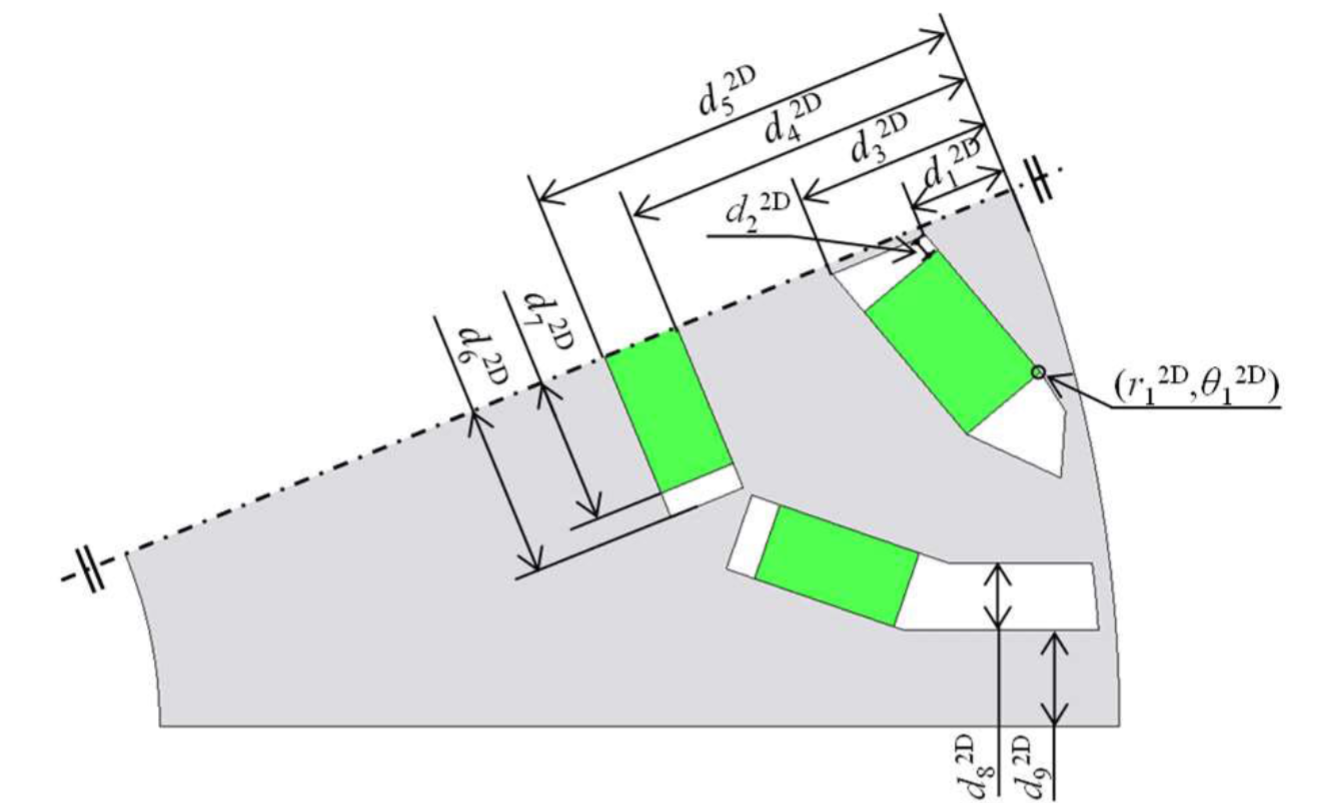
\includegraphics[width=0.5\textwidth]{images/diagram_2d.png}
            \caption{Diagrama do motor 2D.}
            \label{fig:diagram_2d}
        \end{figure}
    \item Nabla
    \\
        \begin{figure}[htbp]
            \centering
            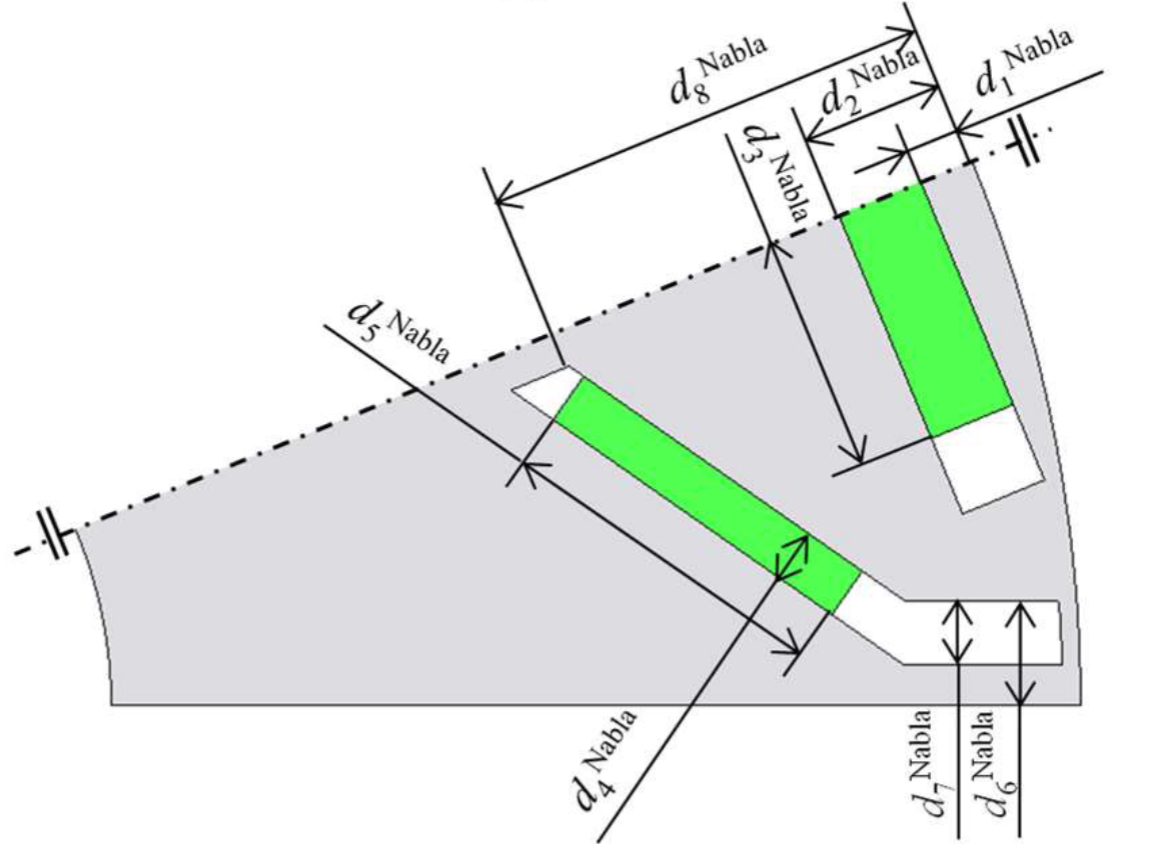
\includegraphics[width=0.5\textwidth]{images/diagram_nabla.png}
            \caption{Diagrama do motor Nabla.}
            \label{fig:diagram_nabla}
        \end{figure}
    \item V
    \\
        \begin{figure}[htbp]
            \centering
            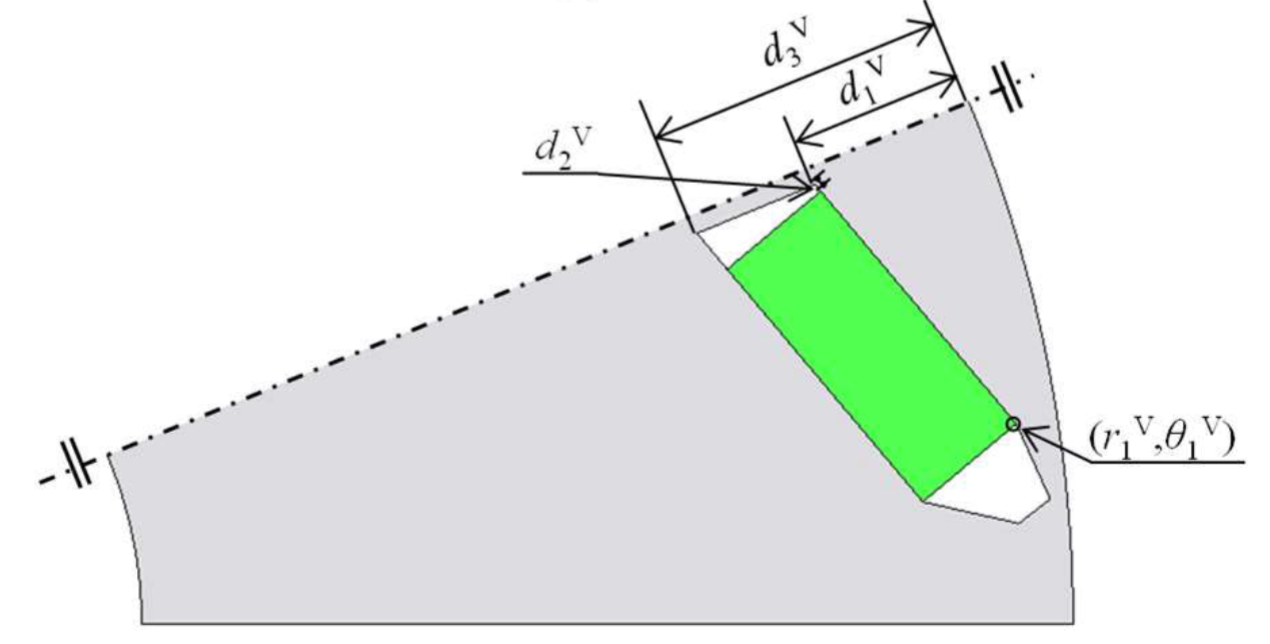
\includegraphics[width=0.5\textwidth]{images/diagram_v.png}
            \caption{Diagrama do motor V.}
            \label{fig:diagram_v}
        \end{figure}
\end{itemize}


\newpage


\subsection{Métricas de Avaliação de Modelos de Regressão}

Para a análise da eficácia de cada modelo na predição dos atributos, foram definidas três métricas\dots

\subsubsection{Mean Absolute Percentage Error (MAPE)}

O \textit{Mean Absolute Percentage Error} (MAPE) mede o erro percentual médio entre
os valores reais $y_i$ e os valores previstos $\hat{y}_i$:

\[
MAPE = \frac{100\%}{n} \sum_{i=1}^{n} \left| \frac{y_i - \hat{y}_i}{y_i} \right|
\]



\subsubsection{Mean Squared Error (MSE)}

O \textit{Mean Squared Error} (MSE) mede o erro quadrático médio, penalizando mais
fortemente desvios grandes:

\[
MSE = \frac{1}{n} \sum_{i=1}^{n} (y_i - \hat{y}_i)^2
\]



\subsubsection{Coeficiente de Determinação ($R^2$)}

O coeficiente de determinação, ou $R^2$, mede a proporção da variância dos dados
reais que é explicada pelo modelo:

\[
R^2 = 1 - \frac{\sum_{i=1}^{n} (y_i - \hat{y}_i)^2}{\sum_{i=1}^{n} (y_i - \bar{y})^2}
\]

onde $\bar{y}$ é a média dos valores reais.


\newpage
% ----------------------------



\subsection{Modelos Utilizados}

Nesta seção, serão apresentados os diferentes modelos de aprendizado de máquina utilizados para a predição. 



\subsubsection{Regressão Linear}

A regressão linear busca modelar a relação entre variáveis de entrada $x_1, x_2, \dots, x_p$ e uma variável de saída $y$, assumindo que essa relação é aproximadamente linear. O modelo é definido por:
\[
\hat{y} = \beta_0 + \sum_{i=1}^p \beta_i x_i,
\]
onde $\beta_0$ é o intercepto e os coeficientes $\beta_i$ representam o peso de cada variável preditora.  

Os parâmetros $\boldsymbol{\beta}$ são estimados pelo método dos mínimos quadrados ordinários (MQO), que minimiza o erro quadrático médio:
\[
\hat{\boldsymbol{\beta}} = \arg \min_{\boldsymbol{\beta}} \sum_{j=1}^n \left(y_j - \beta_0 - \sum_{i=1}^p \beta_i x_{ij}\right)^2.
\]



\subsubsection{Regression Trees}

Uma árvore de regressão divide o espaço das variáveis preditoras em regiões disjuntas $R_1, R_2, \dots, R_M$.  
O modelo pode ser escrito como:
\[
\hat{y}(x) = \sum_{m=1}^M c_m \cdot \mathbb{1}(x \in R_m),
\]
onde $\mathbb{1}(\cdot)$ é a função indicadora, que vale 1 se $x$ pertence à região $R_m$ e 0 caso contrário.  
O valor $c_m$ é geralmente a média dos valores de saída $y$ dos pontos de treino naquela região.



\subsubsection{Random Forests}

O modelo de Random Forests combina $B$ árvores de regressão, cada uma construída a partir de amostras bootstrap dos dados de treino e subconjuntos aleatórios das variáveis. A previsão é a média das árvores:
\[
\hat{y}(x) = \frac{1}{B} \sum_{b=1}^B T_b(x),
\]
onde $T_b(x)$ representa a previsão da $b$-ésima árvore.  



\subsubsection{XGBoost}

O XGBoost é baseado em \textit{gradient boosting}, que combina árvores de forma aditiva para corrigir erros sucessivos. O modelo após $K$ iterações é:
\[
\hat{y}^{(K)}(x) = \sum_{k=1}^K f_k(x), \quad f_k \in \mathcal{F},
\]
onde cada $f_k$ é uma árvore de regressão e $\mathcal{F}$ é o espaço de funções possíveis.  

A cada passo, adiciona-se uma nova árvore $f_k(x)$ para minimizar uma função de perda regularizada:
\[
\mathcal{L}^{(K)} = \sum_{j=1}^n l\big(y_j, \hat{y}^{(K-1)}(x_j) + f_K(x_j)\big) + \Omega(f_K),
\]
onde $l(\cdot)$ é a função de perda (ex.: erro quadrático) e $\Omega(f)$ controla a complexidade do modelo.



\subsubsection{CatBoost}

O CatBoost também segue o princípio do \textit{gradient boosting}, mas introduz técnicas específicas para lidar com variáveis categóricas e reduzir o viés preditivo. Sua formulação geral é semelhante ao XGBoost:
\[
\hat{y}^{(K)}(x) = \sum_{k=1}^K f_k(x),
\]
mas a diferença está no processo de construção das árvores $f_k(x)$, que utiliza estratégias de ordenação para codificação de variáveis categóricas e um esquema de regularização que evita o sobreajuste.


\newpage
% ----------------------


\section{Metodologia}

Para atingir os objetivos deste trabalho, foram definidos 2 experimentos\dots

\subsection{Experimento 1: Identificar os Modelos mais Promissores}

Para esta primeira fase, os hiperparâmetros utilizados foram os já estabelecidos pela linguagem Python, sem nenhuma alteração feita pela pesquisa.

Os modelos de aprendizado foram alimentados com as bases de dados destinadas para treino, X train e y train. Os modelos com target em hysteresis e os com target em joule foram treinados separadamente.

Após essa fase, os dados de X test são fornecidos aos modelos já treinados que retornam, então, os resultados preditos \--- y pred. A acurácia dos modelos é avaliada pela semelhança entre os valores reais em y test e os valores preditos em y pred. Essa acurácia é refletida nas métricas MSE, MAPE e R² score, que foram coletadas ao longo da pesquisa.

Esse processo foi executado com todos os modelos descritos na seção 2.4.

\subsection{Experimento 2: Identificar o melhor conjunto de hiper parâmetros para os modelos mais promissores}

Após o primeiro experimento, foi observado que os dois modelos mais promissores para predição de perdas são XGBoost e CatBoost. Desse modo, há maior chance de que, quando aplicados métodos de hyperparameter tuning, esses modelos retornem resultados mais satisfatórios. Assim, foram determinados os vetores de hiperparâmetros para cada modelo de aprendizado:

\begin{itemize}
    \item Para CatBoost: número de iterações, taxa de aprendizado, profundidade das árvores, regularização L2, força aleatória, temperatura do \textit{bagging}, profundidade máxima das árvores, regularização L1 (\textit{reg\_alpha}) e L2 (\textit{reg\_lambda}).
    \item Para XGBoost: número de árvores (\textit{n\_estimators}), taxa de aprendizado, parâmetro de regularização de divisão (\textit{gamma}), profundidade máxima das árvores, regularização L1 (\textit{reg\_alpha}) e L2 (\textit{reg\_lambda}).
\end{itemize}

Para o alcançe de melhores resultados com menor gasto de processamento, foi utilizado para ambos os modelos o método Randomized Search, que seleciona combinações aletórias entre os valores dos hiperparâmetros, treinando o modelo com cada uma dessas combinações. Em seguida, cada um desses modelos é avaliado segundo a métrica neg MAE (erro médio absoluto negativo) e o melhor conjunto de hiperparâmetros é utilizado para retreinar o modelo final, que retornará o melhor resultado possível.

Também em ambos modelos, foi empregada a técninca de validação cruzada repetida (RepeatedKFold), a fim de obter uma avaliação mais robusta do desempenho.

\newpage

% Resultados
\section{Resultados}

Nesta seção, os resultados para cada motor serão apresentados em 2 formatos: tabelas expondo os valores das métricas e gráficos de comparação entre os valores preditos e os valores reais.

\subsection{Métricas}

\subsubsection{Métricas para o Motor 2D}
% Apresente os resultados obtidos (tabelas, gráficos, análises). Interprete os dados de forma clara e objetiva.

\begin{table}[h!]
\centering
\caption{Métricas para o motor 2D}
\begin{tabular}{llccc}
\toprule
\textbf{method} & \textbf{variable} & \textbf{score} & \textbf{mse} & \textbf{mape} \\
\midrule
\multirow{2}{*}{linear} 
    & hysteresis & 0.877371 & 0.125016 & 0.914328 \\
    & joule      & 0.725346 & 0.316331 & 1.71494 \\
\midrule
\multirow{2}{*}{reg\_tree} 
    & hysteresis & 0.969112 & 0.031489 & 0.549346 \\
    & joule      & 0.822426 & 0.20452 & 0.439176 \\
\midrule
\multirow{2}{*}{rand\_for} 
    & hysteresis & 0.978109 & 0.022318 & 0.315941 \\
    & joule      & 0.831141 & 0.194482 & 0.312343 \\
\midrule
\multirow{2}{*}{catboost} 
    & hysteresis & 0.982187 & 0.018159 & 0.120402 \\
    & joule      & 0.834822 & 0.190243 & 0.192682 \\
\midrule
\multirow{2}{*}{xgboost} 
    & hysteresis & 0.980641 & 0.019735 & 0.191011 \\
    & joule      & 0.833086 & 0.192242 & 0.247595 \\
\midrule
\multirow{2}{*}{cat\_rand} 
    & hysteresis & 0.981849 & 0.018504 & 0.161930 \\
    & joule      & 0.833280 & 0.192019 & 0.196973 \\
\midrule
\multirow{2}{*}{xgb\_rand} 
    & hysteresis & 0.980901 & 0.019471 & 0.178209 \\
    & joule      & 0.833522 & 0.191739 & 0.217464 \\
\bottomrule
\end{tabular}
\end{table}


\subsubsection{Métricas para o Motor Nabla}
% Apresente os resultados obtidos (tabelas, gráficos, análises). Interprete os dados de forma clara e objetiva.

\begin{table}[h!]
\centering
\caption{Métricas para o motor Nabla}
\begin{tabular}{llccc}
\toprule
\textbf{method} & \textbf{variable} & \textbf{score} & \textbf{mse} & \textbf{mape} \\
\midrule
\multirow{2}{*}{linear} 
    & hysteresis & 0.885856 & 0.111261 & 4.135917 \\
    & joule      & 0.851045 & 0.145358 & 1.901598 \\
\midrule
\multirow{2}{*}{reg\_tree} 
    & hysteresis & 0.970236 & 0.029012 & 2.19469 \\
    & joule      & 0.951621 & 0.04721 & 0.954882 \\
\midrule
\multirow{2}{*}{rand\_for} 
    & hysteresis & 0.988997 & 0.010725 & 0.571856 \\
    & joule      & 0.981698 & 0.01786 & 0.50522 \\
\midrule
\multirow{2}{*}{catboost} 
    & hysteresis & 0.995904 & 0.003992 & 0.828559 \\
    & joule      & 0.991773 & 0.008028 & 0.260392 \\
\midrule
\multirow{2}{*}{xgboost} 
    & hysteresis & 0.992065 & 0.007735 & 0.73543 \\
    & joule      & 0.985918 & 0.013741 & 0.424453 \\
\midrule
\multirow{2}{*}{cat\_rand} 
    & hysteresis & 0.995244 &	0.004636 &	0.578424\\
    & joule      & 0.991611 &	0.008186 &	0.268995\\
\midrule
\multirow{2}{*}{xgb\_rand} 
    & hysteresis & 0.993701 &	0.006139 &	0.891864\\
    & joule      &  0.987984 &	0.011726 &	0.298276\\
\bottomrule
\end{tabular}
\end{table}



\subsubsection{Métricas para o Motor V}

\begin{table}[h!]
\centering
\caption{Métricas para o motor V}
\begin{tabular}{llccc}
\toprule
\textbf{method} & \textbf{variable} & \textbf{score} & \textbf{mse} & \textbf{mape} \\
\midrule
\multirow{2}{*}{linear} 
    & hysteresis & 0.898586 & 0.103019 & 1.468986 \\
    & joule      & 0.867551 & 0.134683 & 1.692969 \\
\midrule
\multirow{2}{*}{reg\_tree} 
    & hysteresis & 0.972356 & 0.028081 & 0.687815 \\
    & joule      & 0.972245 & 0.028223 & 0.905085 \\
\midrule
\multirow{2}{*}{rand\_for} 
    & hysteresis & 0.989882 & 0.010278 & 0.57334 \\
    & joule      & 0.989422 & 0.010756 & 0.535394 \\
\midrule
\multirow{2}{*}{catboost} 
    & hysteresis & 0.998258 & 0.00177 & 0.1907 \\
    & joule      & 0.997135 & 0.002913 & 0.318281 \\
\midrule
\multirow{2}{*}{xgboost} 
    & hysteresis & 0.995228 & 0.004847 & 0.428569 \\
    & joule      & 0.993864 & 0.006239 & 0.448335 \\
\midrule
\multirow{2}{*}{cat\_rand} 
    & hysteresis &0.997204 &	0.002841 &	0.263157 \\
    & joule      & 0.996858 &	0.003195 &	0.189069 \\
\midrule
\multirow{2}{*}{xgb\_rand} 
    & hysteresis & 0.995912 &	0.004153 &	0.315962 \\
    & joule      & 0.994688 &	0.005402 &	0.331223 \\
\bottomrule
\end{tabular}
\end{table}

\newpage

\subsection{Gráficos}

\subsubsection{Gráficos para o Motor 2D}

\begin{figure}[!htbp]
    \centering
    % Linha 1: 4 imagens
    \begin{subfigure}[b]{0.23\textwidth}
        \centering
        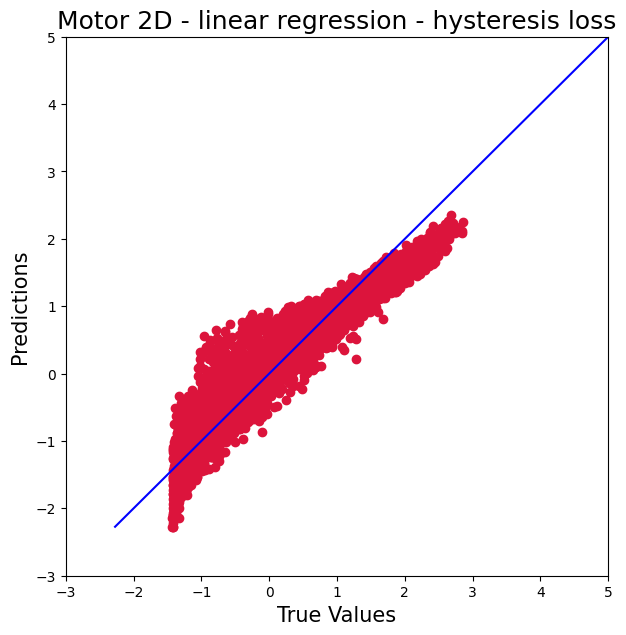
\includegraphics[width=\textwidth]{images/2D/linear_hysteresis.png}
        \caption{Linear Hysteresis}
    \end{subfigure}
    \hfill
    \begin{subfigure}[b]{0.23\textwidth}
        \centering
        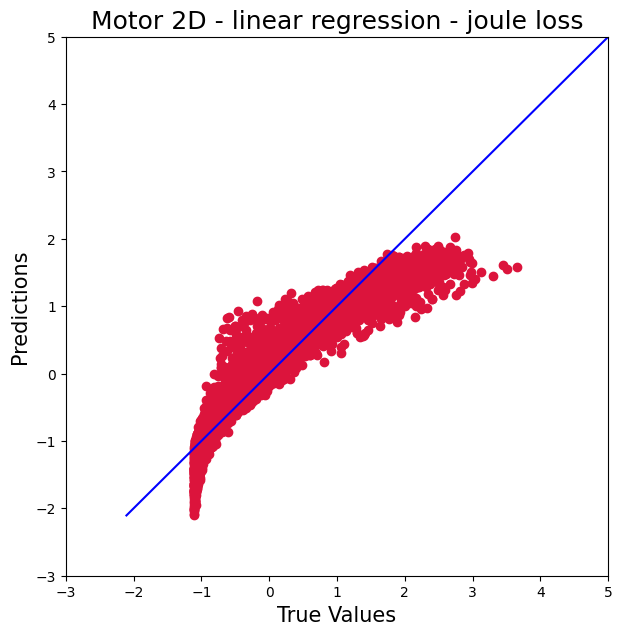
\includegraphics[width=\textwidth]{images/2D/linear_joule.png}
        \caption{Linear Joule}
    \end{subfigure}
    \hfill
    \begin{subfigure}[b]{0.23\textwidth}
        \centering
        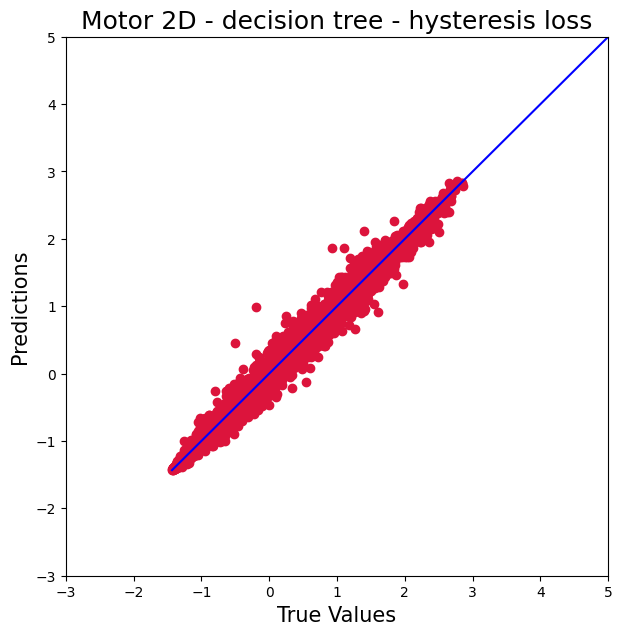
\includegraphics[width=\textwidth]{images/2D/reg_tree_hysteresis.png}
        \caption{Reg Tree Hysteresis}
    \end{subfigure}
    \hfill
    \begin{subfigure}[b]{0.23\textwidth}
        \centering
        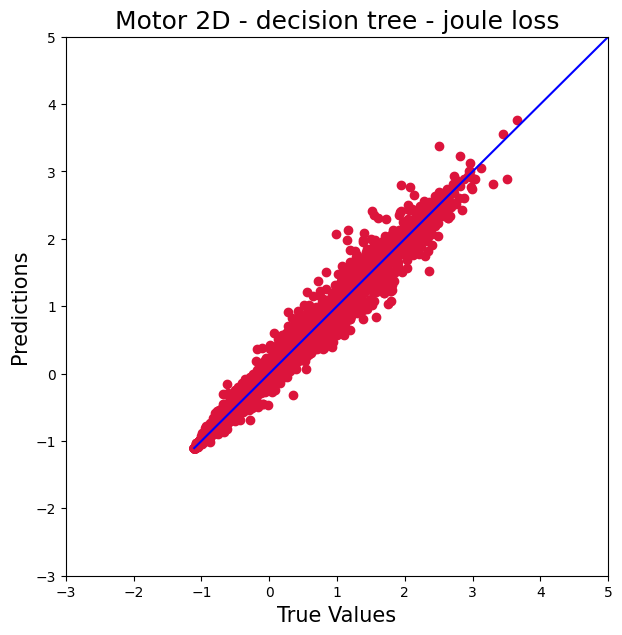
\includegraphics[width=\textwidth]{images/2D/reg_tree_joule.png}
        \caption{Reg Tree Joule}
    \end{subfigure}
    
    \vspace{0.3cm}
    
    % Linha 2: 4 imagens
    \begin{subfigure}[b]{0.23\textwidth}
        \centering
        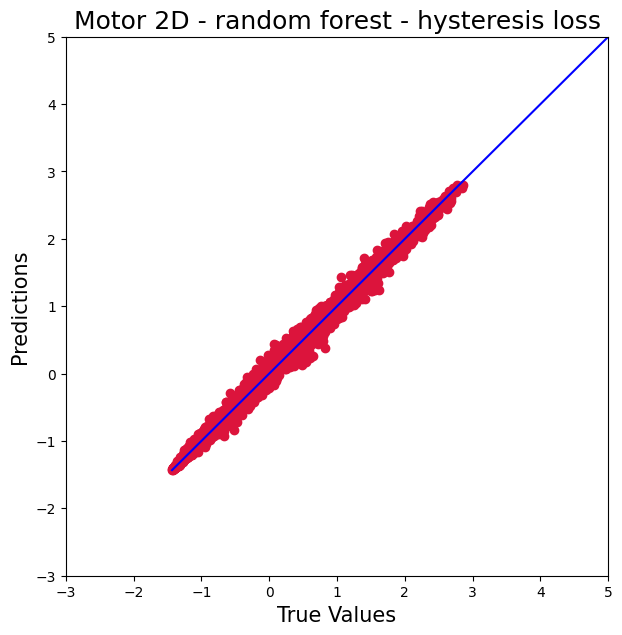
\includegraphics[width=\textwidth]{images/2D/rand_for_hysteresis.png}
        \caption{Rand For Hysteresis}
    \end{subfigure}
    \hfill
    \begin{subfigure}[b]{0.23\textwidth}
        \centering
        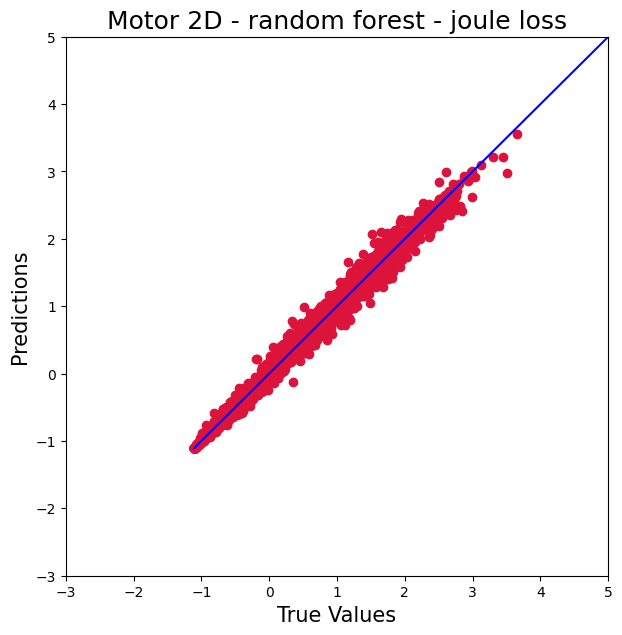
\includegraphics[width=\textwidth]{images/2D/rand_for_joule.png}
        \caption{Rand For Joule}
    \end{subfigure}
    \hfill
    \begin{subfigure}[b]{0.23\textwidth}
        \centering
        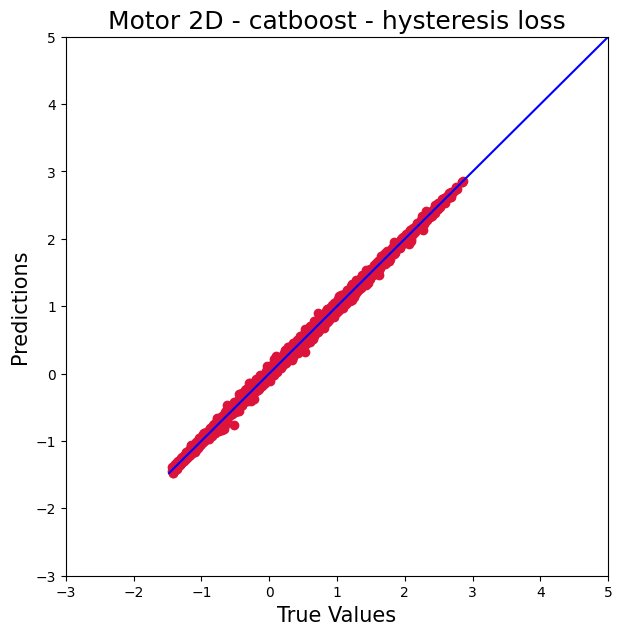
\includegraphics[width=\textwidth]{images/2D/catboost_hysteresis.png}
        \caption{CatBoost Hysteresis}
    \end{subfigure}
    \hfill
    \begin{subfigure}[b]{0.23\textwidth}
        \centering
        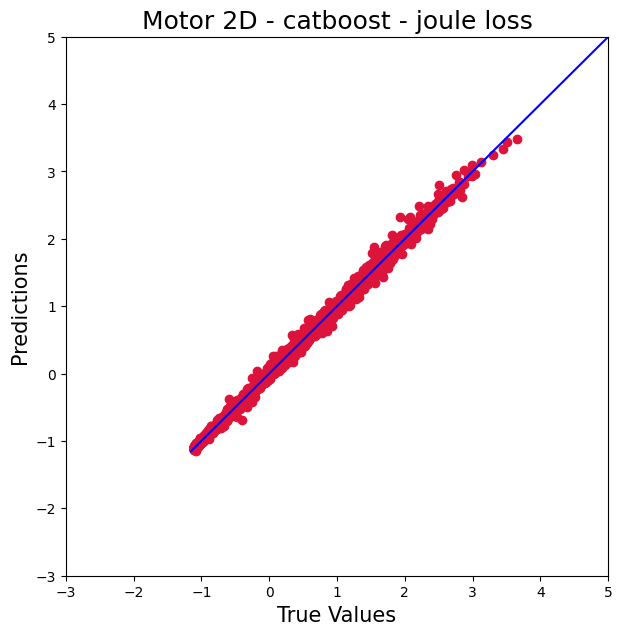
\includegraphics[width=\textwidth]{images/2D/catboost_joule.png}
        \caption{CatBoost Joule}
    \end{subfigure}
    
    \vspace{0.3cm}
    
    % Linha 3: 4 imagens
    \begin{subfigure}[b]{0.23\textwidth}
        \centering
        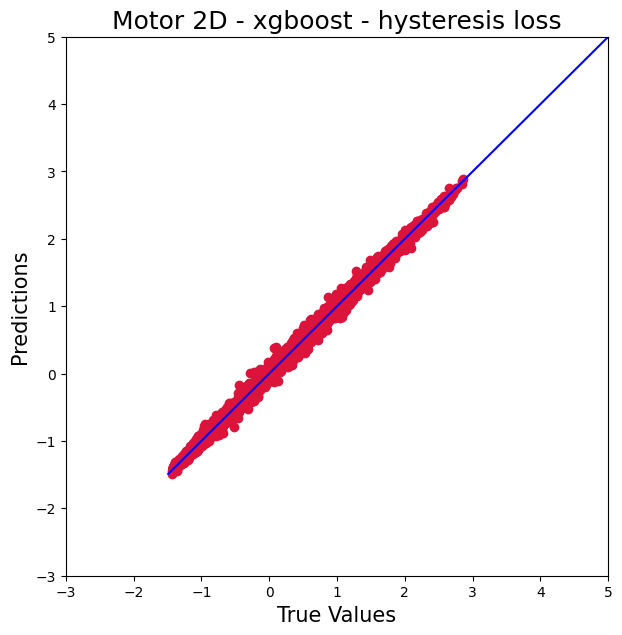
\includegraphics[width=\textwidth]{images/2D/xgboost_hysteresis.png}
        \caption{XGBoost Hysteresis}
    \end{subfigure}
    \hfill
    \begin{subfigure}[b]{0.23\textwidth}
        \centering
        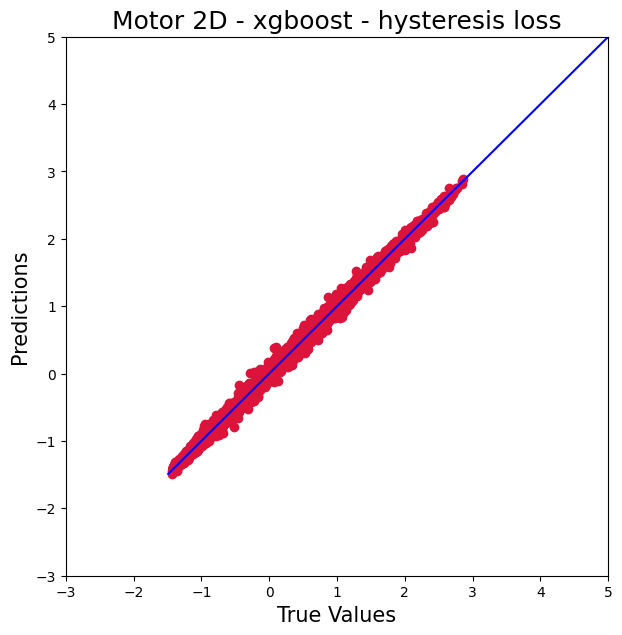
\includegraphics[width=\textwidth]{images/2D/xgboost_joule.png}
        \caption{XGBoost Joule}
    \end{subfigure}
    \hfill
    \begin{subfigure}[b]{0.23\textwidth}
        \centering
        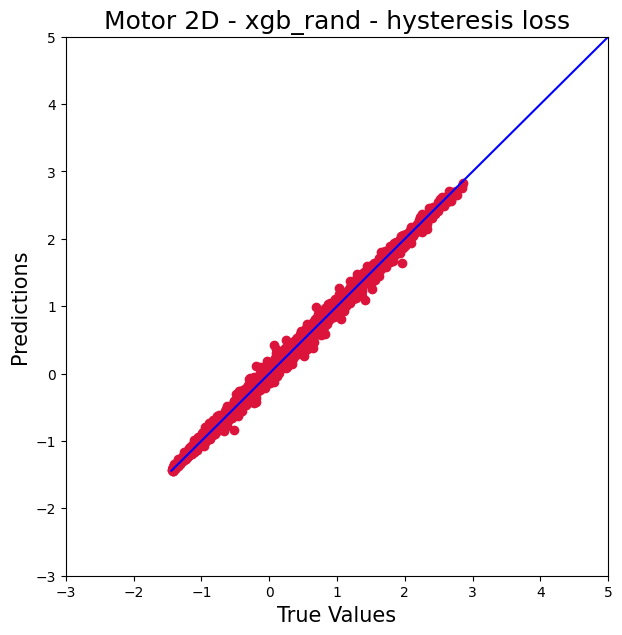
\includegraphics[width=\textwidth]{images/2D/xgb_rand_hysteresis.png}
        \caption{XGB Rand Hysteresis}
    \end{subfigure}
    \hfill
    \begin{subfigure}[b]{0.23\textwidth}
        \centering
        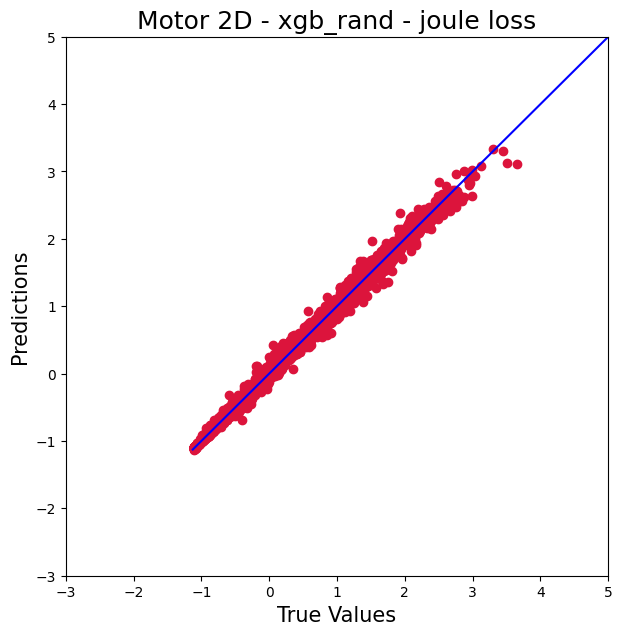
\includegraphics[width=\textwidth]{images/2D/xgb_rand_joule.png}
        \caption{XGB Rand Joule}
    \end{subfigure}
    
    \vspace{0.3cm}
    
    % Linha 4: 2 imagens (centralizadas)
    \begin{subfigure}[b]{0.23\textwidth}
        \centering
        \null
    \end{subfigure}
    \hfill
    \centering
    \begin{subfigure}[b]{0.23\textwidth}
        \centering
        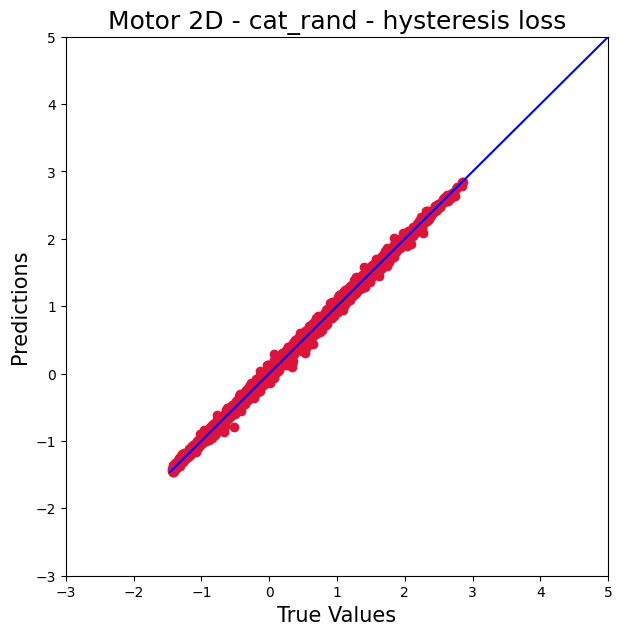
\includegraphics[width=\textwidth]{images/2D/cat_rand_hysteresis.png}
        \caption{Cat Rand Hysteresis}
    \end{subfigure}
    \hfill
    \begin{subfigure}[b]{0.23\textwidth}
        \centering
        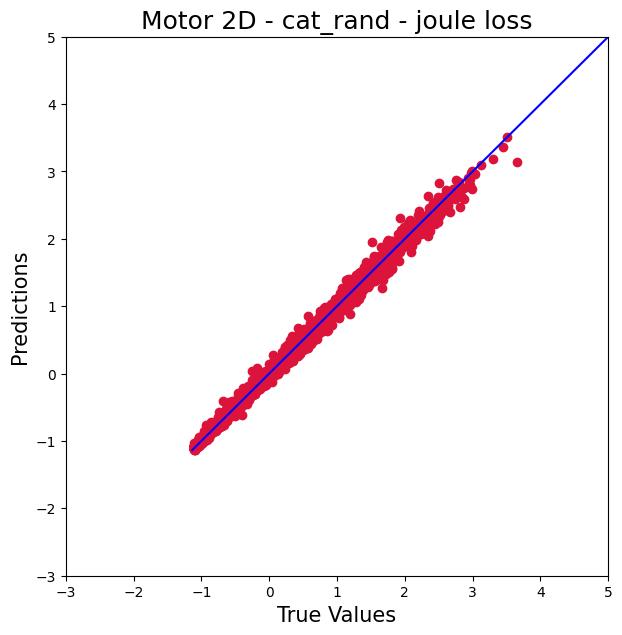
\includegraphics[width=\textwidth]{images/2D/cat_rand_joule.png}
        \caption{Cat Rand Joule}
    \end{subfigure}
    \hfill
    % Espaços vazios para manter o alinhamento
    \begin{subfigure}[b]{0.23\textwidth}
        \centering
        \null
    \end{subfigure}
    
    \caption{Comparação entre resultados para o motor 2D.}
\end{figure}



\newpage

\subsubsection{Gráficos para o Motor Nabla}

\begin{figure}[!htbp]
    \centering
    % Linha 1: 4 imagens
    \begin{subfigure}[b]{0.23\textwidth}
        \centering
        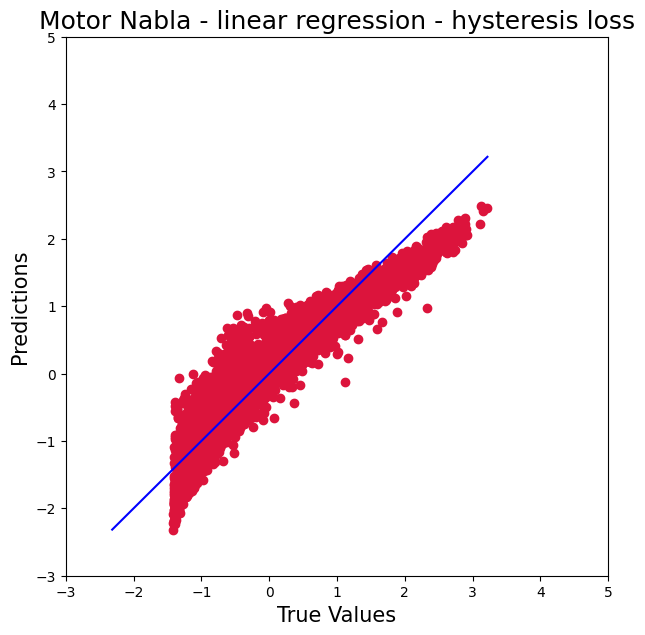
\includegraphics[width=\textwidth]{images/Nabla/linear_hysteresis.png}
        \caption{Linear Hysteresis}
    \end{subfigure}
    \hfill
    \begin{subfigure}[b]{0.23\textwidth}
        \centering
        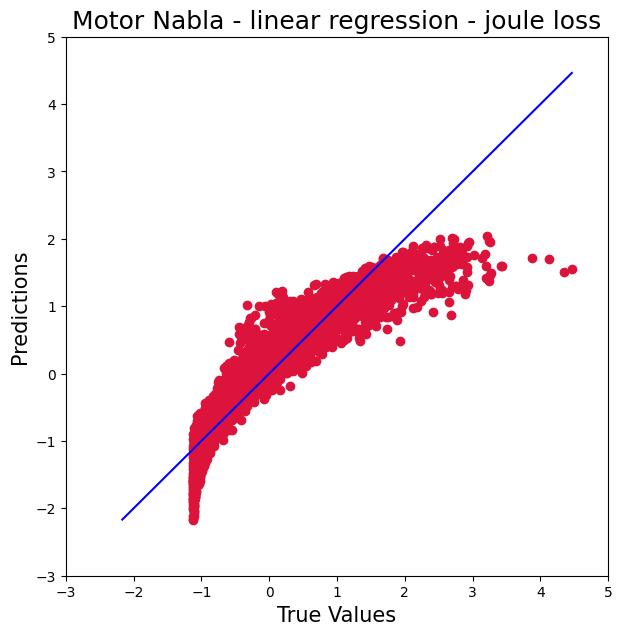
\includegraphics[width=\textwidth]{images/Nabla/linear_joule.png}
        \caption{Linear Joule}
    \end{subfigure}
    \hfill
    \begin{subfigure}[b]{0.23\textwidth}
        \centering
        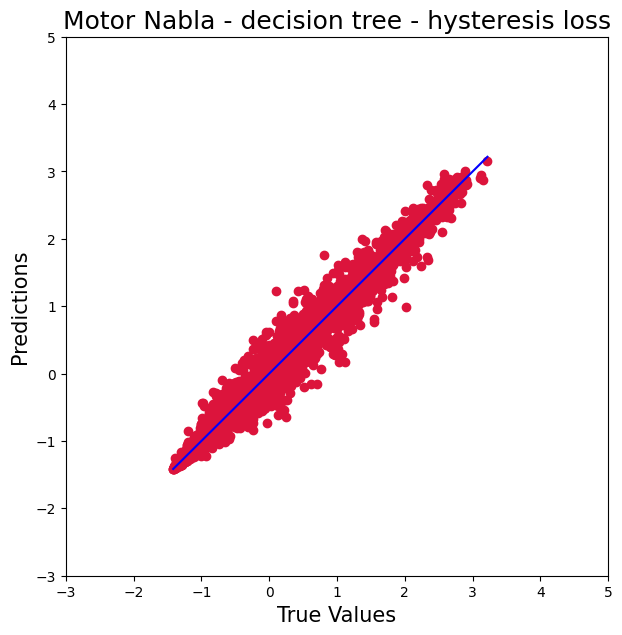
\includegraphics[width=\textwidth]{images/Nabla/reg_tree_hysteresis.png}
        \caption{Reg Tree Hysteresis}
    \end{subfigure}
    \hfill
    \begin{subfigure}[b]{0.23\textwidth}
        \centering
        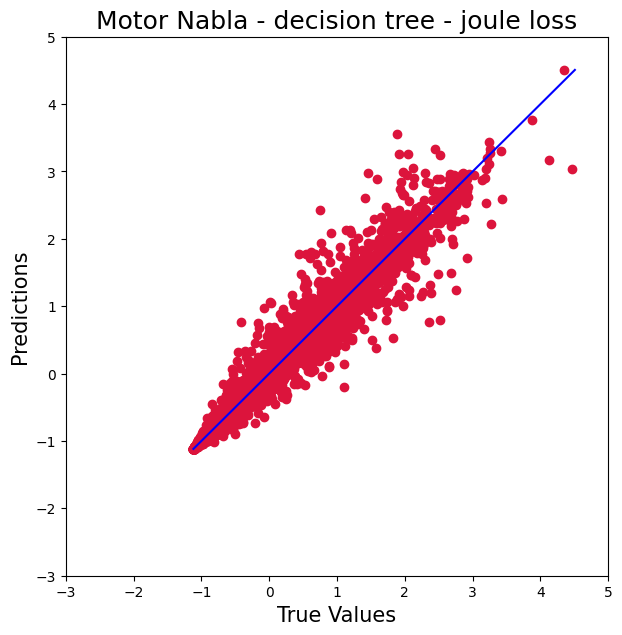
\includegraphics[width=\textwidth]{images/Nabla/reg_tree_joule.png}
        \caption{Reg Tree Joule}
    \end{subfigure}
    
    \vspace{0.3cm}
    
    % Linha 2: 4 imagens
    \begin{subfigure}[b]{0.23\textwidth}
        \centering
        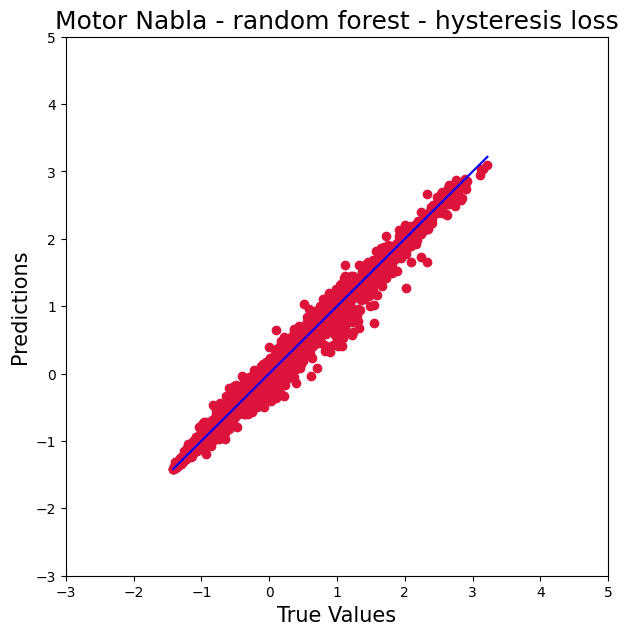
\includegraphics[width=\textwidth]{images/Nabla/rand_for_hysteresis.png}
        \caption{Rand For Hysteresis}
    \end{subfigure}
    \hfill
    \begin{subfigure}[b]{0.23\textwidth}
        \centering
        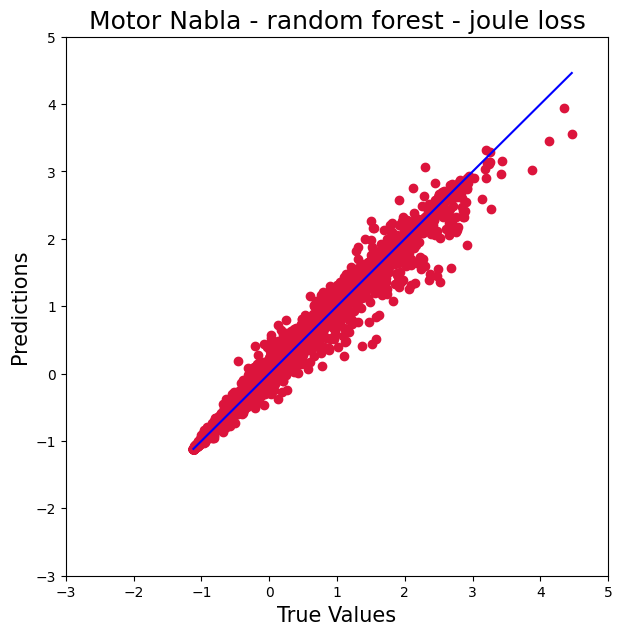
\includegraphics[width=\textwidth]{images/Nabla/rand_for_joule.png}
        \caption{Rand For Joule}
    \end{subfigure}
    \hfill
    \begin{subfigure}[b]{0.23\textwidth}
        \centering
        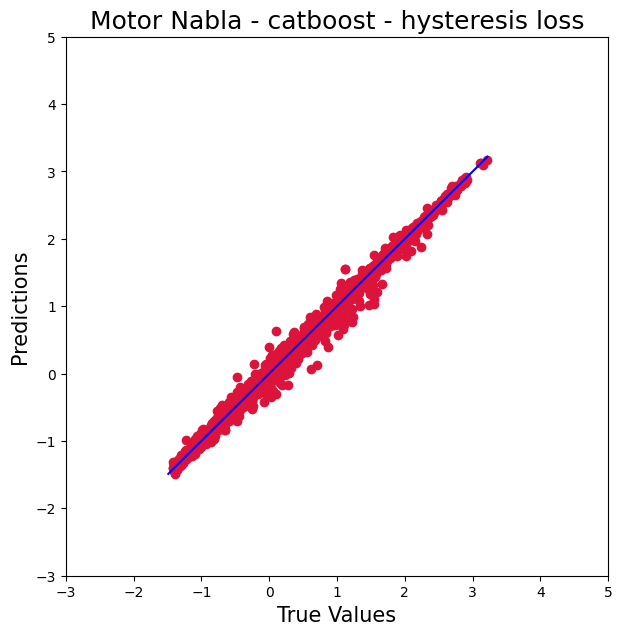
\includegraphics[width=\textwidth]{images/Nabla/catboost_hysteresis.png}
        \caption{CatBoost Hysteresis}
    \end{subfigure}
    \hfill
    \begin{subfigure}[b]{0.23\textwidth}
        \centering
        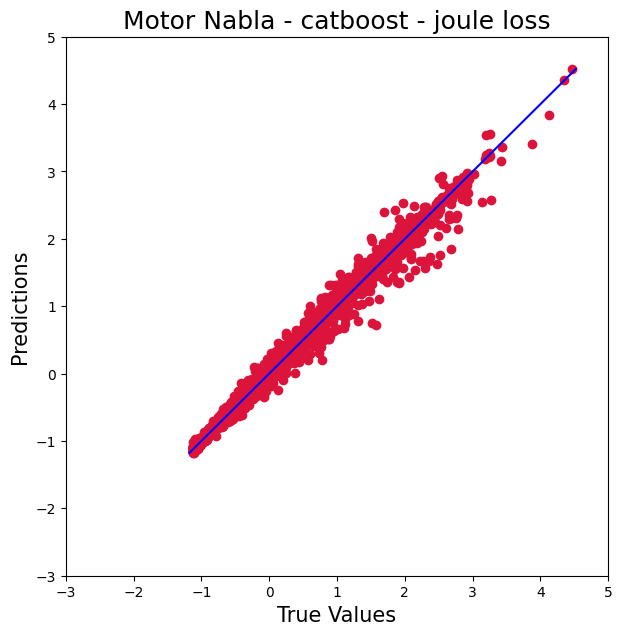
\includegraphics[width=\textwidth]{images/Nabla/catboost_joule.png}
        \caption{CatBoost Joule}
    \end{subfigure}
    
    \vspace{0.3cm}
    
    % Linha 3: 4 imagens
    \begin{subfigure}[b]{0.23\textwidth}
        \centering
        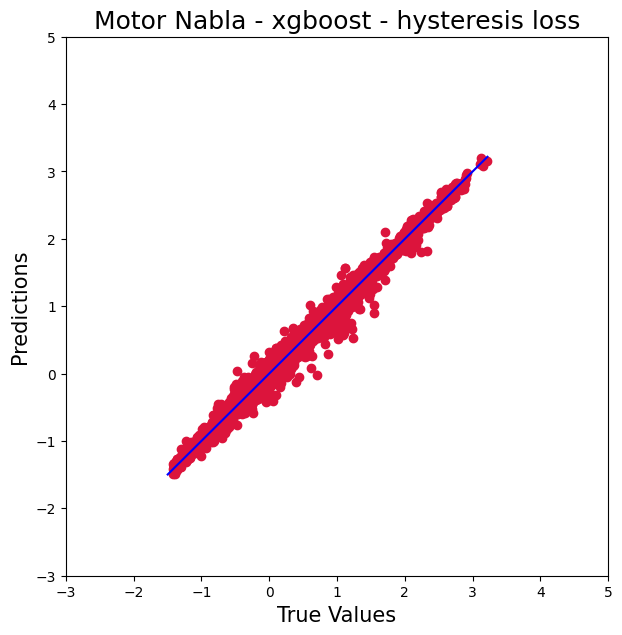
\includegraphics[width=\textwidth]{images/Nabla/xgboost_hysteresis.png}
        \caption{XGBoost Hysteresis}
    \end{subfigure}
    \hfill
    \begin{subfigure}[b]{0.23\textwidth}
        \centering
        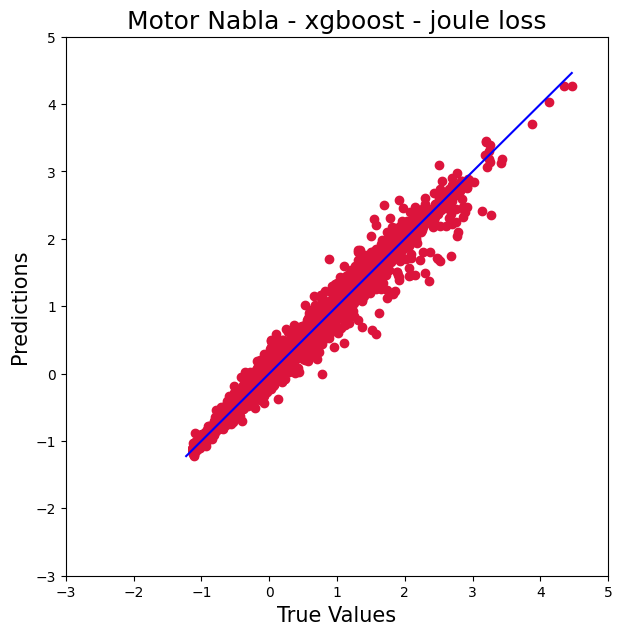
\includegraphics[width=\textwidth]{images/Nabla/xgboost_joule.png}
        \caption{XGBoost Joule}
    \end{subfigure}
    \hfill
    \begin{subfigure}[b]{0.23\textwidth}
        \centering
        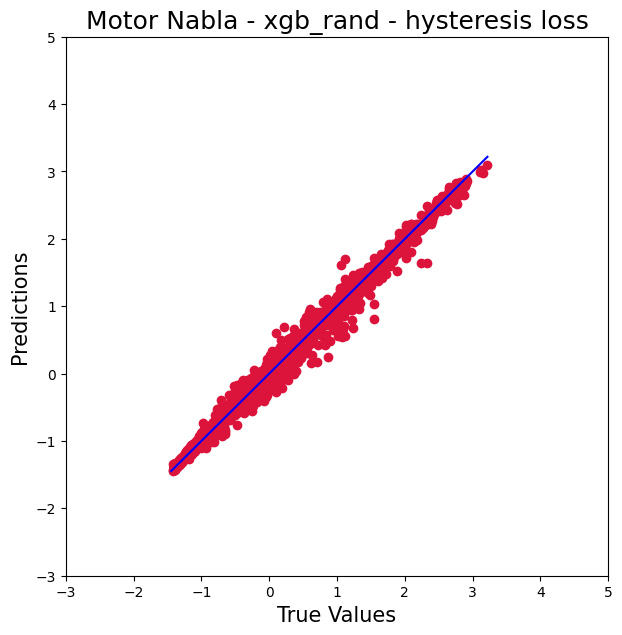
\includegraphics[width=\textwidth]{images/Nabla/xgb_rand_hysteresis.png}
        \caption{XGB Rand Hysteresis}
    \end{subfigure}
    \hfill
    \begin{subfigure}[b]{0.23\textwidth}
        \centering
        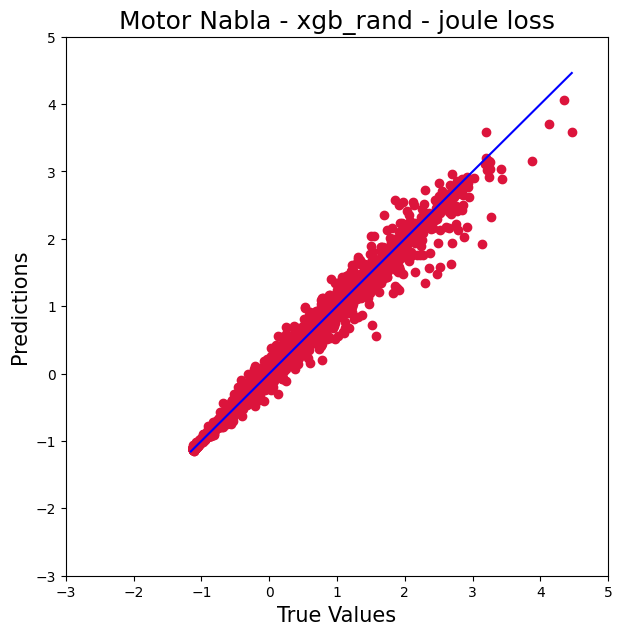
\includegraphics[width=\textwidth]{images/Nabla/xgb_rand_joule.png}
        \caption{XGB Rand Joule}
    \end{subfigure}
    
    \vspace{0.3cm}
    
    % Linha 4: 2 imagens (centralizadas)
    \begin{subfigure}[b]{0.23\textwidth}
        \centering
        \null
    \end{subfigure}
    \hfill
    \centering
    \begin{subfigure}[b]{0.23\textwidth}
        \centering
        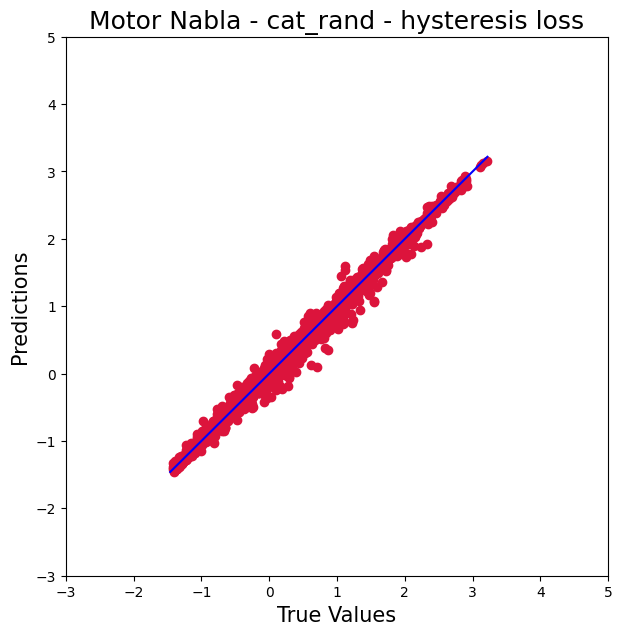
\includegraphics[width=\textwidth]{images/Nabla/cat_rand_hysteresis.png}
        \caption{Cat Rand Hysteresis}
    \end{subfigure}
    \hfill
    \begin{subfigure}[b]{0.23\textwidth}
        \centering
        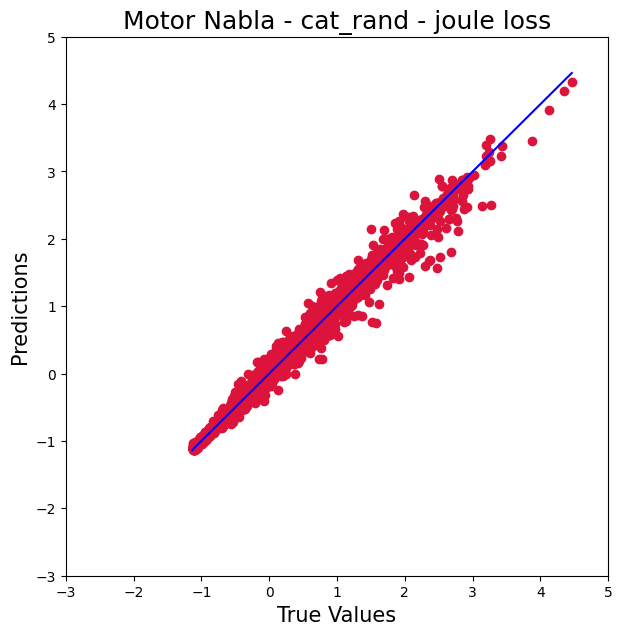
\includegraphics[width=\textwidth]{images/Nabla/cat_rand_joule.png}
        \caption{Cat Rand Joule}
    \end{subfigure}
    \hfill
    % Espaços vazios para manter o alinhamento
    \begin{subfigure}[b]{0.23\textwidth}
        \centering
        \null
    \end{subfigure}
    
    \caption{Comparação entre resultados para o motor Nabla.}
\end{figure}

\newpage

\subsubsection{Gráficos para o Motor V}

\begin{figure}[!htbp]
    \centering
    % Linha 1: 4 imagens
    \begin{subfigure}[b]{0.23\textwidth}
        \centering
        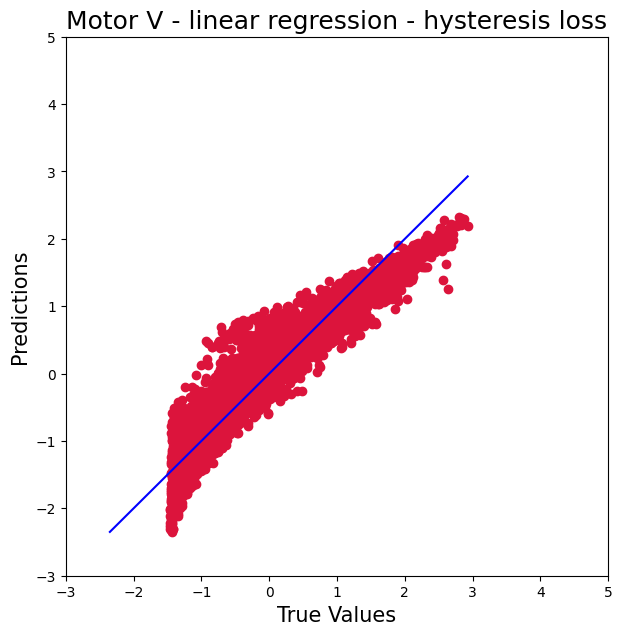
\includegraphics[width=\textwidth]{images/V/linear_hysteresis.png}
        \caption{Linear Hysteresis}
    \end{subfigure}
    \hfill
    \begin{subfigure}[b]{0.23\textwidth}
        \centering
        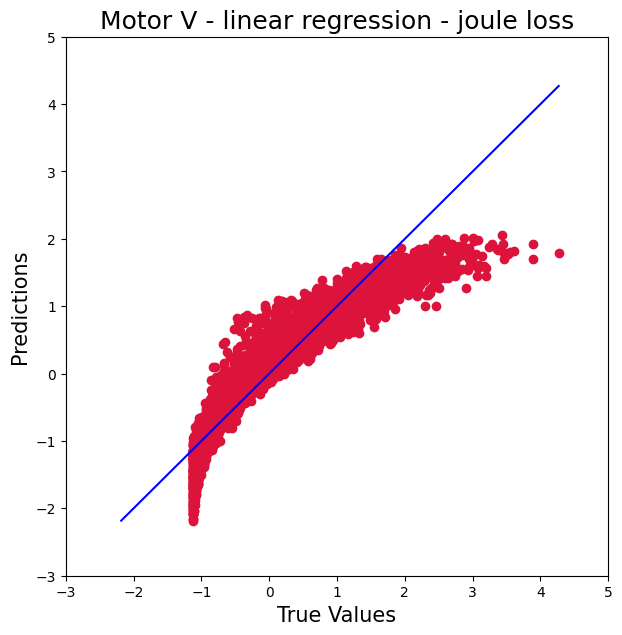
\includegraphics[width=\textwidth]{images/V/linear_joule.png}
        \caption{Linear Joule}
    \end{subfigure}
    \hfill
    \begin{subfigure}[b]{0.23\textwidth}
        \centering
        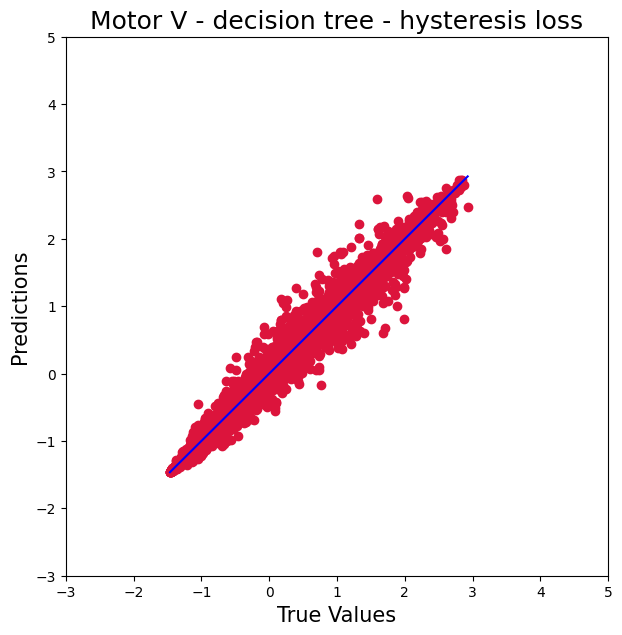
\includegraphics[width=\textwidth]{images/V/reg_tree_hysteresis.png}
        \caption{Reg Tree Hysteresis}
    \end{subfigure}
    \hfill
    \begin{subfigure}[b]{0.23\textwidth}
        \centering
        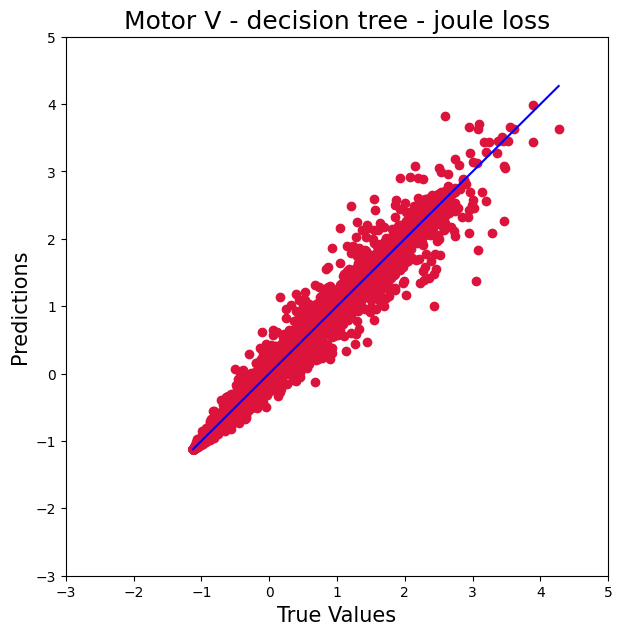
\includegraphics[width=\textwidth]{images/V/reg_tree_joule.png}
        \caption{Reg Tree Joule}
    \end{subfigure}
    
    \vspace{0.3cm}
    
    % Linha 2: 4 imagens
    \begin{subfigure}[b]{0.23\textwidth}
        \centering
        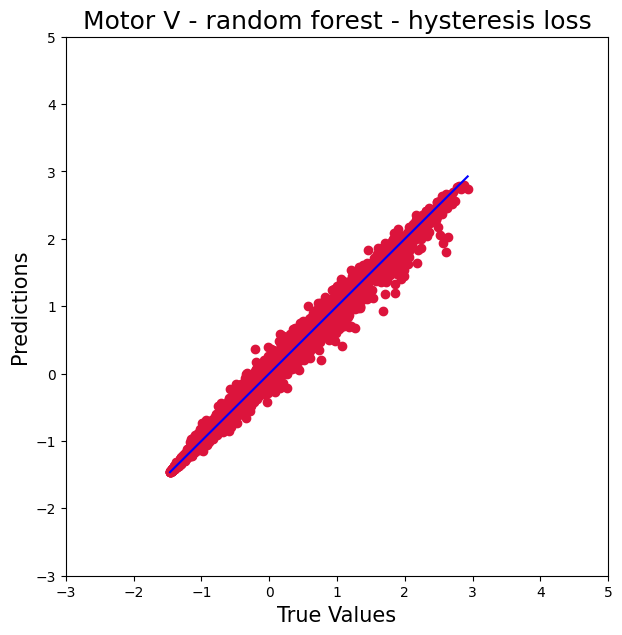
\includegraphics[width=\textwidth]{images/V/rand_for_hysteresis.png}
        \caption{Rand For Hysteresis}
    \end{subfigure}
    \hfill
    \begin{subfigure}[b]{0.23\textwidth}
        \centering
        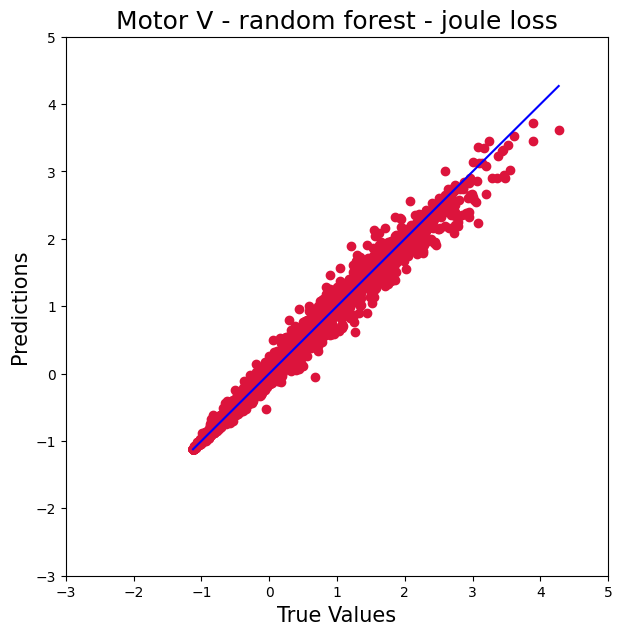
\includegraphics[width=\textwidth]{images/V/rand_for_joule.png}
        \caption{Rand For Joule}
    \end{subfigure}
    \hfill
    \begin{subfigure}[b]{0.23\textwidth}
        \centering
        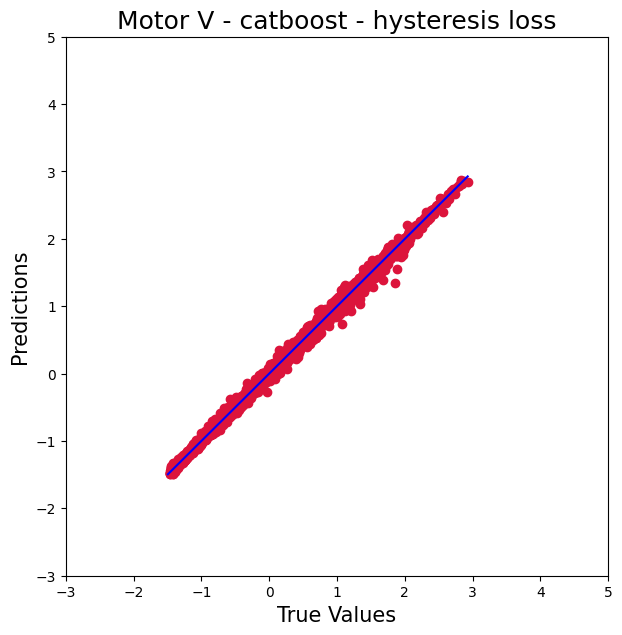
\includegraphics[width=\textwidth]{images/V/catboost_hysteresis.png}
        \caption{CatBoost Hysteresis}
    \end{subfigure}
    \hfill
    \begin{subfigure}[b]{0.23\textwidth}
        \centering
        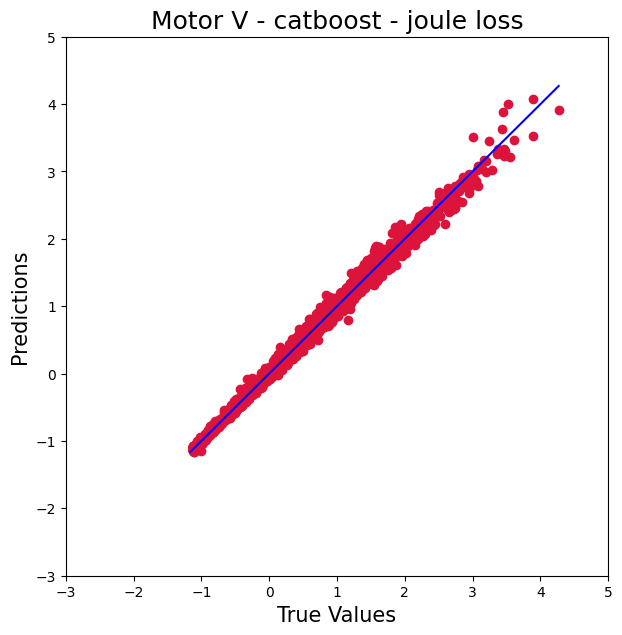
\includegraphics[width=\textwidth]{images/V/catboost_joule.png}
        \caption{CatBoost Joule}
    \end{subfigure}
    
    \vspace{0.3cm}
    
    % Linha 3: 4 imagens
    \begin{subfigure}[b]{0.23\textwidth}
        \centering
        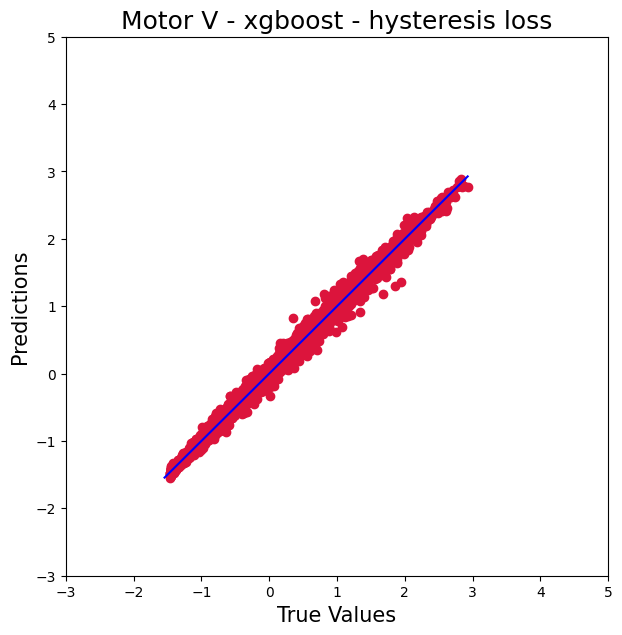
\includegraphics[width=\textwidth]{images/V/xgboost_hysteresis.png}
        \caption{XGBoost Hysteresis}
    \end{subfigure}
    \hfill
    \begin{subfigure}[b]{0.23\textwidth}
        \centering
        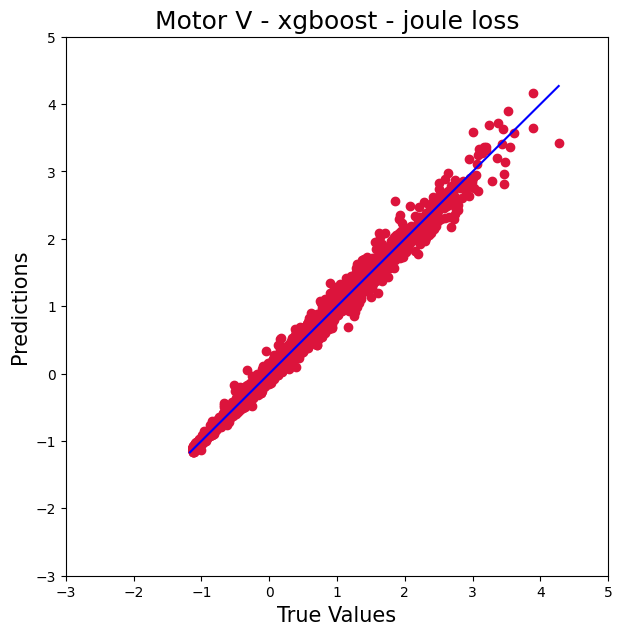
\includegraphics[width=\textwidth]{images/V/xgboost_joule.png}
        \caption{XGBoost Joule}
    \end{subfigure}
    \hfill
    \begin{subfigure}[b]{0.23\textwidth}
        \centering
        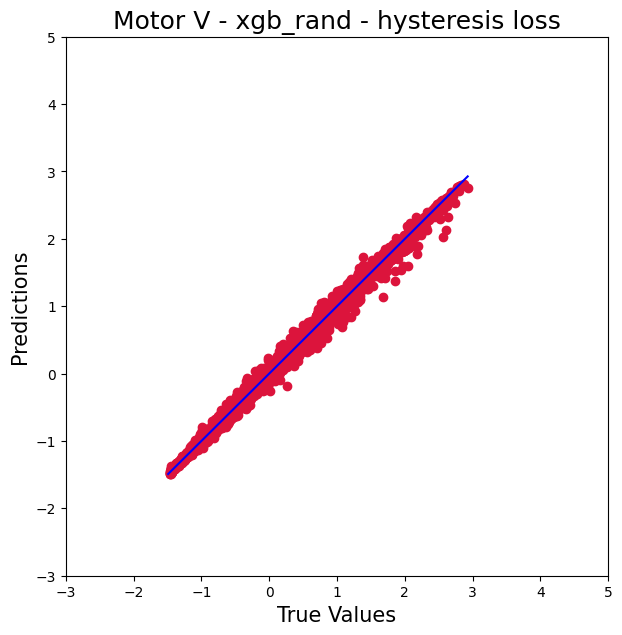
\includegraphics[width=\textwidth]{images/V/xgb_rand_hysteresis.png}
        \caption{XGB Rand Hysteresis}
    \end{subfigure}
    \hfill
    \begin{subfigure}[b]{0.23\textwidth}
        \centering
        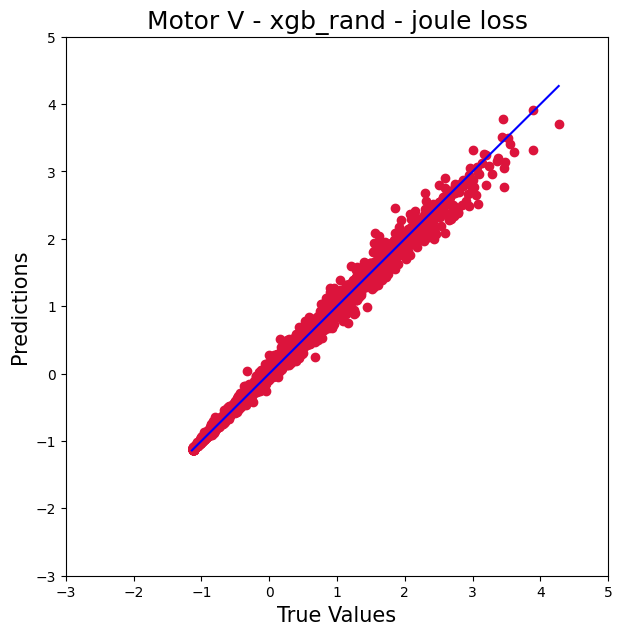
\includegraphics[width=\textwidth]{images/V/xgb_rand_joule.png}
        \caption{XGB Rand Joule}
    \end{subfigure}
    
    \vspace{0.3cm}
    
    % Linha 4: 2 imagens (centralizadas)
    \begin{subfigure}[b]{0.23\textwidth}
        \centering
        \null
    \end{subfigure}
    \hfill
    \centering
    \begin{subfigure}[b]{0.23\textwidth}
        \centering
        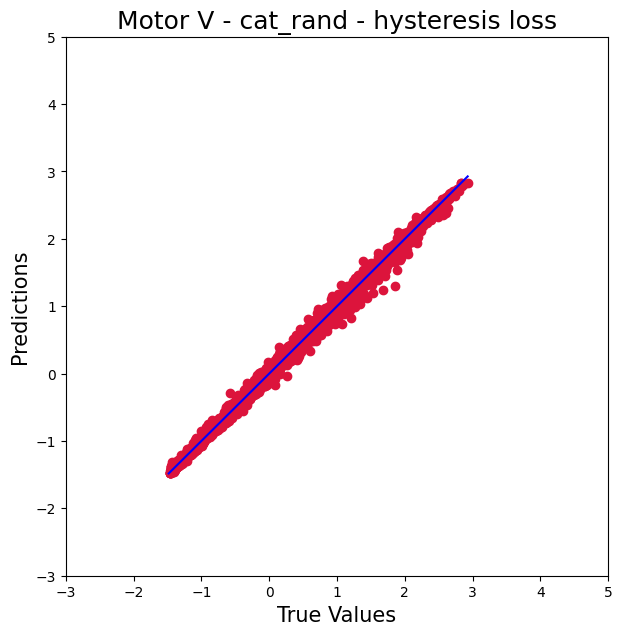
\includegraphics[width=\textwidth]{images/V/cat_rand_hysteresis.png}
        \caption{Cat Rand Hysteresis}
    \end{subfigure}
    \hfill
    \begin{subfigure}[b]{0.23\textwidth}
        \centering
        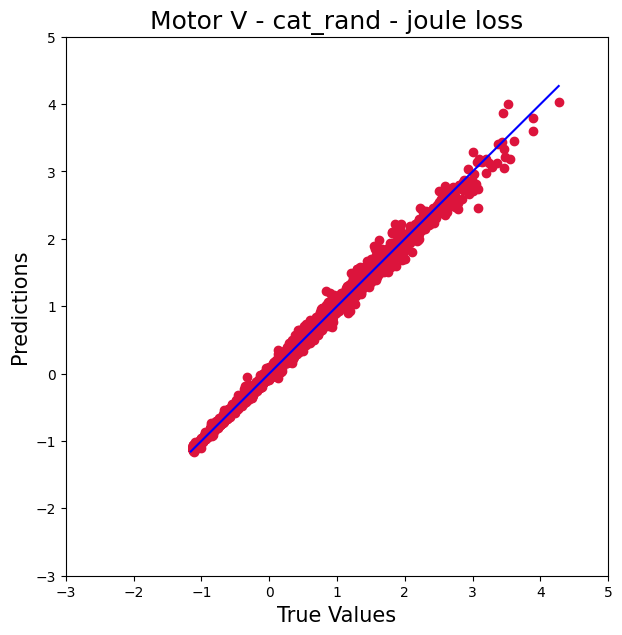
\includegraphics[width=\textwidth]{images/V/cat_rand_joule.png}
        \caption{Cat Rand Joule}
    \end{subfigure}
    \hfill
    % Espaços vazios para manter o alinhamento
    \begin{subfigure}[b]{0.23\textwidth}
        \centering
        \null
    \end{subfigure}
    
    \caption{Comparação entre resultados para o motor V.}
\end{figure}

\newpage

\subsection{Observações}

No geral, a predição da perda por histerese retornou melhores resultados quando comparados à predição de perda por joule.

Como esperado, o modelo de regressão linear provou-se como o menos eficaz para a predição de valores dos \textit{targets}. Isso se deve, muito provavelmente, ao fato de que a regressão linear é um modelo extremamente simples e rudimentar.

Dentre os modelos observados na primeira fase experimental, destacam-se 2: \textit{CatBoost} e \textit{XGBoost}. Contudo, observa-se que os resultados obtidos com \textit{CatBoost} foram ainda mais satisfatórios.

Já na segunda fase experimental, o comportamento do método \textit{Randomized Search} foi errático. Em alguns casos, houve uma melhora substancial nos resultados, quando comparados àqueles obtidos com modelos sem ajustes nos hiperparâmetros. Em outros, o comportamento foi contrário, e uma leve piora foi registrada. Isso pode ser explicado pela utilização dos mesmos hiperparâmetros e métodos para modelos em diferentes conjuntos de dados.

Nota-se que o motor 2D obteve os melhores valores para MAPE dentre todos os outros motores. Entretanto, seu coeficiente de determinação e MSE não refletiram valores tão positivos quanto os demais. Na comparação entre valores preditos e observados, é notável que os resultados de 2D também se sobressaíram.

% Conclusão
\section{Conclusão}

Tendo em mãos os resultados inesperados em alguns dos modelos, como valores piores na predição de perda por \textit{eddy current} e métricas flutuantes para o motor 2D, vale pontuar a importância de melhor análise das razões destes comportamentos em trabalhos futuros.

Em relação à escolha dos modelos de aprendizado, é evidente que \textit{CatBoost} e \textit{XGBoost} são promissores. Para este tipo de problema e de base de dados, o uso dos modelos rudimentares como \textit{Linear Regression}, \textit{Regression Tree} e \textit{Random Forest} não provou gerar resultados positivos.

Além disso, o estudo de hiperparâmetros e melhores configurações pode ser vantajoso para obter modelos mais precisos. 

\newpage
\section{Referências}
% \printbibliography

\end{document}
